\documentclass[12pt]{article}\usepackage[]{graphicx}\usepackage[]{color}
%% maxwidth is the original width if it is less than linewidth
%% otherwise use linewidth (to make sure the graphics do not exceed the margin)
\makeatletter
\def\maxwidth{ %
  \ifdim\Gin@nat@width>\linewidth
    \linewidth
  \else
    \Gin@nat@width
  \fi
}
\makeatother

\definecolor{fgcolor}{rgb}{0.345, 0.345, 0.345}
\newcommand{\hlnum}[1]{\textcolor[rgb]{0.686,0.059,0.569}{#1}}%
\newcommand{\hlstr}[1]{\textcolor[rgb]{0.192,0.494,0.8}{#1}}%
\newcommand{\hlcom}[1]{\textcolor[rgb]{0.678,0.584,0.686}{\textit{#1}}}%
\newcommand{\hlopt}[1]{\textcolor[rgb]{0,0,0}{#1}}%
\newcommand{\hlstd}[1]{\textcolor[rgb]{0.345,0.345,0.345}{#1}}%
\newcommand{\hlkwa}[1]{\textcolor[rgb]{0.161,0.373,0.58}{\textbf{#1}}}%
\newcommand{\hlkwb}[1]{\textcolor[rgb]{0.69,0.353,0.396}{#1}}%
\newcommand{\hlkwc}[1]{\textcolor[rgb]{0.333,0.667,0.333}{#1}}%
\newcommand{\hlkwd}[1]{\textcolor[rgb]{0.737,0.353,0.396}{\textbf{#1}}}%
\let\hlipl\hlkwb

\usepackage{framed}
\makeatletter
\newenvironment{kframe}{%
 \def\at@end@of@kframe{}%
 \ifinner\ifhmode%
  \def\at@end@of@kframe{\end{minipage}}%
  \begin{minipage}{\columnwidth}%
 \fi\fi%
 \def\FrameCommand##1{\hskip\@totalleftmargin \hskip-\fboxsep
 \colorbox{shadecolor}{##1}\hskip-\fboxsep
     % There is no \\@totalrightmargin, so:
     \hskip-\linewidth \hskip-\@totalleftmargin \hskip\columnwidth}%
 \MakeFramed {\advance\hsize-\width
   \@totalleftmargin\z@ \linewidth\hsize
   \@setminipage}}%
 {\par\unskip\endMakeFramed%
 \at@end@of@kframe}
\makeatother

\definecolor{shadecolor}{rgb}{.97, .97, .97}
\definecolor{messagecolor}{rgb}{0, 0, 0}
\definecolor{warningcolor}{rgb}{1, 0, 1}
\definecolor{errorcolor}{rgb}{1, 0, 0}
\newenvironment{knitrout}{}{} % an empty environment to be redefined in TeX

\usepackage{alltt}
 
\usepackage[margin=1in]{geometry}
\usepackage{amsmath,amsthm,amssymb, mathtools}
\usepackage[T1]{fontenc}
\usepackage{lmodern}
\usepackage{fixltx2e}
\usepackage[shortlabels]{enumitem}
 
\newcommand{\N}{\mathbb{N}}
\newcommand{\R}{\mathbb{R}}
\newcommand{\Z}{\mathbb{Z}}
\newcommand{\Q}{\mathbb{Q}}
 
\newenvironment{theorem}[2][Theorem]{\begin{trivlist}
\item[\hskip \labelsep {\bfseries #1}\hskip \labelsep {\bfseries #2.}]}{\end{trivlist}}
\newenvironment{lemma}[2][Lemma]{\begin{trivlist}
\item[\hskip \labelsep {\bfseries #1}\hskip \labelsep {\bfseries #2.}]}{\end{trivlist}}
\newenvironment{exercise}[2][Exercise]{\begin{trivlist}
\item[\hskip \labelsep {\bfseries #1}\hskip \labelsep {\bfseries #2.}]}{\end{trivlist}}
\newenvironment{problem}[2][Problem]{\begin{trivlist}
\item[\hskip \labelsep {\bfseries #1}\hskip \labelsep {\bfseries #2.}]}{\end{trivlist}}
\newenvironment{question}[2][Question]{\begin{trivlist}
\item[\hskip \labelsep {\bfseries #1}\hskip \labelsep {\bfseries #2.}]}{\end{trivlist}}
\newenvironment{corollary}[2][Corollary]{\begin{trivlist}
\item[\hskip \labelsep {\bfseries #1}\hskip \labelsep {\bfseries #2.}]}{\end{trivlist}}
\newcommand{\textfrac}[2]{\dfrac{\text{#1}}{\text{#2}}}
\IfFileExists{upquote.sty}{\usepackage{upquote}}{}
\begin{document}

\title{Statistical Rethinking: Chapter 4 - Linear Models}

\author{Chris Hayduk}
\date{\today}

\maketitle




\section{Easy}

\begin{problem}{4E1}
\text{ }\\
In the model definition below, which line is the likelihood?
\begin{enumerate}
	\item y\textsubscript{i} $\sim$ Normal($\mu$, $\sigma$)
	\item $\mu$ $\sim$ Normal(0, 10)
	\item $\sigma$ $\sim$ Uniform(0, 10)
\end{enumerate}
\end{problem}

Line 1 represents the likelihood.

\begin{problem}{4E2}
\text{ }\\
In the model definition just above, how many parameters are in the posterior distribution?
\end{problem}

There are two parameters: $\mu$ and $\sigma$.

\begin{problem}{4E3}
\text{ }\\
Using the model definition above, write down the appropriate form of Bayes' theorem that includes the proper likelihood and priors.
\end{problem}

Pr($\mu$, $\sigma$\vert$y) = \textfrac{$\Pi$\textsubscript{i}Normal(y\textsubscript{i}$\vert$\mu$, $\sigma$) Normal($\mu$\vert$0, 10) Uniform($\sigma$\vert$0, 10)}{$\int$\int$\Pi$\textsubscript{i}Normal(y\textsubscript{i}$\vert$\mu$, $\sigma$) Normal($\mu$\vert$0, 10) Uniform($\sigma$\vert$0, 10) $\textit{d}$\mu$\textit{d}$\sigma$}

\begin{problem}{4E4}
\text{ }\\
In the model definition below, which line is the linear model?
\begin{enumerate}
	\item y\textsubscript{i} $\sim$ Normal($\mu$, $\sigma$)
	\item $\mu$\textsubscript{i} = $\alpha$ + $\beta$x\textsubscript{i}
	\item $\alpha$ $\sim$ Normal(0, 10)
	\item $\beta$ $\sim$ Normal(0, 10)
	\item $\sigma$ $\sim$ Uniform(0, 10)
\end{enumerate}
\end{problem}

Line 2 represents the linear model.

\begin{problem}{4E5}
\text{ }\\
In the model definition just above, how many parameters are in the posterior distribution?
\end{problem}

There are three parameters: $\alpha$, $\beta$, and $\sigma$.

\section{Medium}

\begin{problem}{4M1}
\text{}\\
For the model definition below, simulate the observed heights from the prior (not the posterior).
\begin{center}
y\textsubscript{i} $\sim$ Normal($\mu$, $\sigma$)\\
$\mu$ $\sim$ Normal(0, 10)\\
$\sigma$ $\sim$ Uniform(0, 10)
\end{center}
\end{problem}

\begin{knitrout}
\definecolor{shadecolor}{rgb}{0.969, 0.969, 0.969}\color{fgcolor}\begin{kframe}
\begin{alltt}
\hlstd{sample_mu} \hlkwb{<-} \hlkwd{rnorm}\hlstd{(}\hlnum{1e4}\hlstd{,} \hlnum{0}\hlstd{,} \hlnum{10}\hlstd{)}
\hlstd{sample_sigma} \hlkwb{<-} \hlkwd{runif}\hlstd{(}\hlnum{1e4}\hlstd{,} \hlnum{0}\hlstd{,} \hlnum{10}\hlstd{)}
\hlstd{prior_h} \hlkwb{<-} \hlkwd{rnorm}\hlstd{(}\hlnum{1e4}\hlstd{, sample_mu, sample_sigma)}
\hlkwd{dens}\hlstd{(prior_h)}
\end{alltt}
\end{kframe}
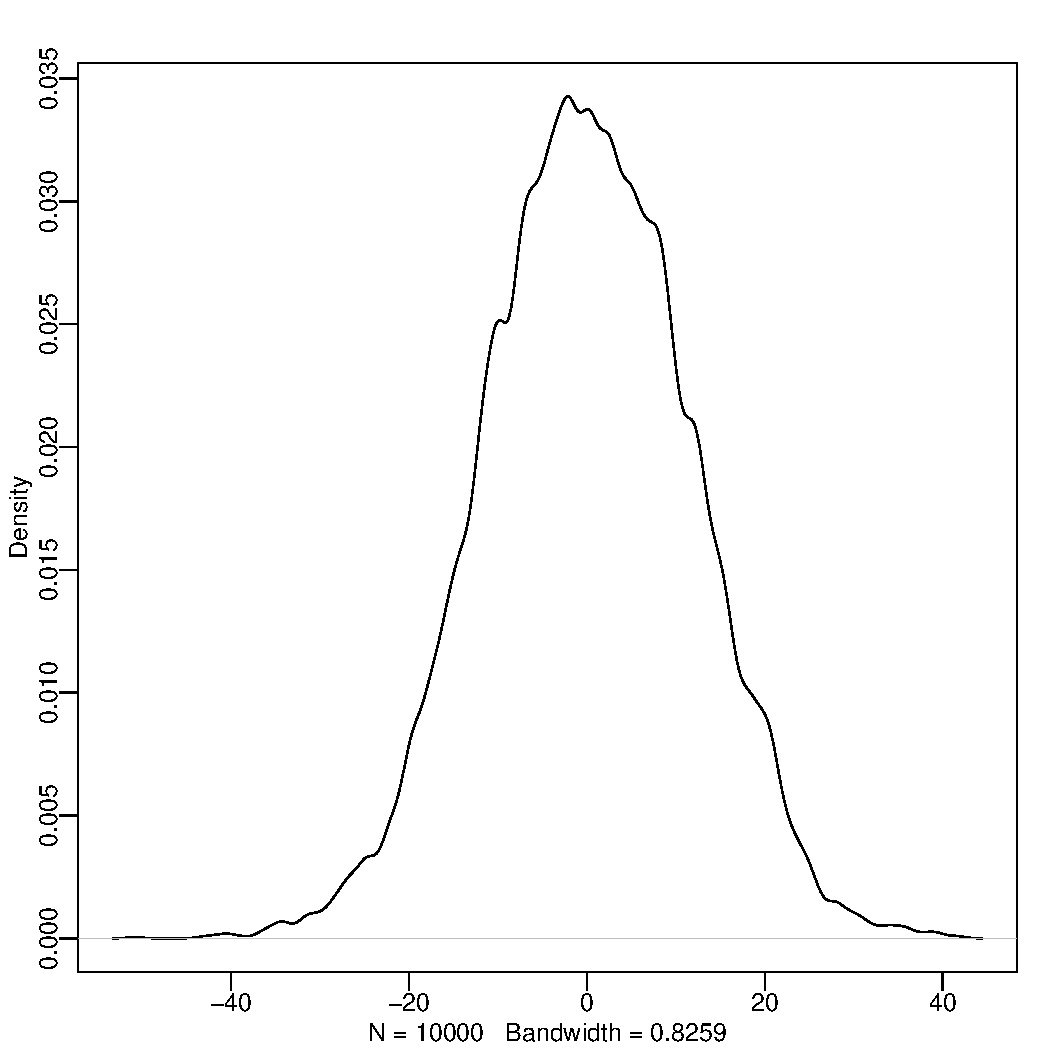
\includegraphics[width=\maxwidth]{figure/unnamed-chunk-2-1} 

\end{knitrout}

\begin{problem}{4M2}
\text{}\\
Translate the model just above into a \textit{map} formula.
\end{problem}

\begin{knitrout}
\definecolor{shadecolor}{rgb}{0.969, 0.969, 0.969}\color{fgcolor}\begin{kframe}
\begin{alltt}
\hlstd{flist} \hlkwb{<-} \hlkwd{alist}\hlstd{(}
  \hlstd{y} \hlopt{~} \hlkwd{dnorm}\hlstd{(mu, sigma),}
  \hlstd{mu} \hlopt{~} \hlkwd{dnorm}\hlstd{(}\hlnum{0}\hlstd{,} \hlnum{10}\hlstd{),}
  \hlstd{sigma} \hlopt{~} \hlkwd{dunif}\hlstd{(}\hlnum{0}\hlstd{,} \hlnum{10}\hlstd{)}
\hlstd{)}
\end{alltt}
\end{kframe}
\end{knitrout}

\begin{problem}{4M3}
\text{}\\
Translate the \textit{map} model formula below into a mathematical model definition.

\begin{knitrout}
\definecolor{shadecolor}{rgb}{0.969, 0.969, 0.969}\color{fgcolor}\begin{kframe}
\begin{alltt}
\hlstd{flist} \hlkwb{<-} \hlkwd{alist}\hlstd{(}
  \hlstd{y} \hlopt{~} \hlkwd{dnorm}\hlstd{(mu, sigma),}
  \hlstd{mu} \hlkwb{<-} \hlstd{a} \hlopt{+}\hlstd{b}\hlopt{*}\hlstd{x,}
  \hlstd{a} \hlopt{~} \hlkwd{dnorm}\hlstd{(}\hlnum{0}\hlstd{,} \hlnum{50}\hlstd{),}
  \hlstd{b} \hlopt{~} \hlkwd{dunif}\hlstd{(}\hlnum{0}\hlstd{,} \hlnum{10}\hlstd{),}
  \hlstd{sigma} \hlopt{~} \hlkwd{dunif}\hlstd{(}\hlnum{0}\hlstd{,} \hlnum{50}\hlstd{)}
\hlstd{)}
\end{alltt}
\end{kframe}
\end{knitrout}
\end{problem}

Model:
\begin{center}
y\textsubscript{i} $\sim$ Normal($\mu$, $\sigma$)\\
$\mu$\textsubscript{i} = $\alpha$ + $\beta$x\textsubscript{i}\\
$\alpha$ $\sim$ Normal(0, 50)\\
$\beta$ $\sim$ Uniform(0, 10)\\
$\sigma$ $\sim$ Uniform(0, 50)
\end{center}

\begin{problem}{4M4}
\text{}\\
A sample of students is measured for height each year for 3 years. After the third year, you want to fit a linear regression predicting height using year as a predictor. Write down the mathematical model for this regression, using any variable names and priors you choose. Be prepared to defend your choice of priors.
\end{problem}

Model:
\begin{center}
y\textsubscript{i} $\sim$ Normal($\mu$, $\sigma$)\\
$\mu$\textsubscript{i} = $\alpha$ + $\beta$x\textsubscript{i}\\
$\alpha$ $\sim$ Normal(152, 25)\\
$\beta$ $\sim$ Normal(6, 3)\\
$\sigma$ $\sim$ Uniform(0, 50)
\end{center}

The priors for $\alpha$ represent an average of about 5 feet (152 cm) and a standard deviation of about 10 inches (25 cm).
The priors for $\beta$ represent an average increase of about 2.4 inches per year (6 cm - chosen using average growth rate for children) and a standard deviation of about 1.19 inches (3 cm).
The prior for $\sigma$ is a uniform prior between 0 and 50.

\begin{problem}{4M5}
\text{}\\
Now suppose I tell you that the average height in the first year was 120 cm and that every student got taller each year and every student got taller each year. Does this information lead you to change your choice of prior?
\end{problem}

With this no information, we should adjust $\alpha$. We now have:
\begin{center}
y\textsubscript{i} $\sim$ Normal($\mu$, $\sigma$)\\
$\mu$\textsubscript{i} = $\alpha$ + $\beta$x\textsubscript{i}\\
$\alpha$ $\sim$ Normal(120, 25)\\
$\beta$ $\sim$ Normal(6, 3)\\
$\sigma$ $\sim$ Uniform(0, 50)
\end{center}

The priors for $\alpha$ have been adjusted to account for the new information we have about the average height in the first year.
We already chose $\beta$ as a positive number with a relatively small standard deviation, so the information about students growing taller each year does not effect our choice of prior.

\begin{problem}{4M6}
\text{}\\
Now suppose I tell you that the variance among heights for students of the same age is never more than 64 cm. How does this lead you to revise your priors?
\end{problem}

$\sigma$ is just the square root of the variance. Thus, we would like $\beta$'s standard deviation to be less than $\sqrt{64}=8$. Since we already chose a standard deviation of 3 cm, we do not need to revise this choice.

\section{Hard}

\begin{problem}{4H1}
\text{}\\
The weights listed below were recorded in the !Kung census, but heights were not recorded for these individuals. Provide predicted heights and 89\% intervals (either HPDI or PI) for each of these individuals. That is, fill in the table below, using model-based predictions.
\end{problem}

\begin{knitrout}
\definecolor{shadecolor}{rgb}{0.969, 0.969, 0.969}\color{fgcolor}\begin{kframe}
\begin{alltt}
\hlkwd{data}\hlstd{(Howell1)}

\hlstd{d1} \hlkwb{<-} \hlstd{Howell1}

\hlstd{m1} \hlkwb{<-} \hlkwd{map}\hlstd{(}
  \hlkwd{alist}\hlstd{(}
    \hlstd{height} \hlopt{~} \hlkwd{dnorm}\hlstd{(a} \hlopt{+} \hlstd{b}\hlopt{*}\hlstd{weight, sigma),}
    \hlstd{a} \hlopt{~} \hlkwd{dnorm}\hlstd{(}\hlnum{178}\hlstd{,} \hlnum{100}\hlstd{),}
    \hlstd{b} \hlopt{~} \hlkwd{dnorm}\hlstd{(}\hlnum{0}\hlstd{,} \hlnum{10}\hlstd{),}
    \hlstd{sigma} \hlopt{~} \hlkwd{dunif}\hlstd{(}\hlnum{0}\hlstd{,} \hlnum{50}\hlstd{)}
  \hlstd{),} \hlkwc{data} \hlstd{= d1)}

\hlstd{weights} \hlkwb{<-} \hlkwd{c}\hlstd{(}\hlnum{46.95}\hlstd{,} \hlnum{43.72}\hlstd{,} \hlnum{64.78}\hlstd{,} \hlnum{32.59}\hlstd{,} \hlnum{54.63}\hlstd{)}

\hlstd{sim.height} \hlkwb{<-} \hlkwd{sim}\hlstd{(m1,} \hlkwc{data}\hlstd{=}\hlkwd{list}\hlstd{(}\hlkwc{weight}\hlstd{=weights),} \hlkwc{n} \hlstd{=} \hlnum{1e4}\hlstd{,} \hlkwc{silent} \hlstd{=} \hlnum{TRUE}\hlstd{)}
\end{alltt}
\begin{verbatim}
## [ 1000 / 10000 ]
[ 2000 / 10000 ]
[ 3000 / 10000 ]
[ 4000 / 10000 ]
[ 5000 / 10000 ]
[ 6000 / 10000 ]
[ 7000 / 10000 ]
[ 8000 / 10000 ]
[ 9000 / 10000 ]
[ 10000 / 10000 ]

\end{verbatim}
\begin{alltt}
\hlstd{mean.height} \hlkwb{<-} \hlkwd{apply}\hlstd{(sim.height,} \hlnum{2}\hlstd{, mean)}

\hlkwd{print}\hlstd{(mean.height)}
\end{alltt}
\begin{verbatim}
## [1] 158.3036 152.4159 189.8263 132.8623 171.8030
\end{verbatim}
\begin{alltt}
\hlstd{height.PI} \hlkwb{<-} \hlkwd{apply}\hlstd{(sim.height,} \hlnum{2}\hlstd{, PI,} \hlkwc{prob}\hlstd{=}\hlnum{0.89}\hlstd{)}

\hlkwd{print}\hlstd{(height.PI)}
\end{alltt}
\begin{verbatim}
##         [,1]     [,2]     [,3]     [,4]     [,5]
## 5%  143.4731 137.5300 174.5770 117.9404 156.6272
## 94% 172.9770 167.1276 205.0343 147.6429 186.8567
\end{verbatim}
\end{kframe}
\end{knitrout}

\begin{center}
 \begin{tabular}{||c c c c||} 
 \hline
 Individual & weight & expected height & 89\% interval \\ [0.5ex] 
 \hline\hline
 1 & 46.95 & 158.43 & (143.67, 173.42) \\ 
 \hline
 2 & 43.72 & 152.56 & (137.83, 167.69) \\
 \hline
 3 & 64.78 & 189.54 & (174.28, 204.93) \\
 \hline
 4 & 32.59 & 133.09 & (118.25, 148.41) \\
 \hline
 5 & 54.63 & 171.67 & (156.48, 186.94) \\ [1ex] 
 \hline
\end{tabular}
\end{center}

\begin{problem}{4H2}
\text{}\\
Select out all the rows in the Howell1 data with ages below 18 years of age. If you do it right, you should end up with a new data frame with 192 rows in it.
\begin{enumerate}[(a)]
\item Fit a linear regression to these data, using \textit{map}. Present and interpret the estimates. For every 10 units of increase in weight, how much taller does the model predict a child gets?
\item Plot the raw data, with height on the vertical axis and weight on the horizontal axis. Superimpose the MAP regression line and 89\% HPDI for the mean. Also superimpose the 89\% HPDI for predicted heights.
\item What aspects of the model fit concern you? Describe the kinds of assumptions you would change, if any, to improve the model. You don't have to write any new code. Just explain what the model appears to be doing a bad job of, and what you hypothesize would be a better model.
\end{enumerate}
\end{problem}
\\
\begin{enumerate}[(a)]
\item 

\begin{knitrout}
\definecolor{shadecolor}{rgb}{0.969, 0.969, 0.969}\color{fgcolor}\begin{kframe}
\begin{alltt}
\hlstd{d2} \hlkwb{<-} \hlstd{Howell1}
\hlstd{d2} \hlkwb{<-} \hlstd{d2[d2}\hlopt{$}\hlstd{age} \hlopt{<} \hlnum{18}\hlstd{, ]}

\hlkwd{str}\hlstd{(d2)}
\end{alltt}
\begin{verbatim}
## 'data.frame':	192 obs. of  4 variables:
##  $ height: num  121.9 105.4 86.4 129.5 109.2 ...
##  $ weight: num  19.6 13.9 10.5 23.6 16 ...
##  $ age   : num  12 8 6.5 13 7 17 16 11 17 8 ...
##  $ male  : int  1 0 0 1 0 1 0 1 0 1 ...
\end{verbatim}
\begin{alltt}
\hlstd{m2} \hlkwb{<-} \hlkwd{map}\hlstd{(}
  \hlkwd{alist}\hlstd{(}
    \hlstd{height} \hlopt{~} \hlkwd{dnorm}\hlstd{(a} \hlopt{+} \hlstd{b}\hlopt{*}\hlstd{weight, sigma),}
    \hlstd{a} \hlopt{~} \hlkwd{dnorm}\hlstd{(}\hlnum{178}\hlstd{,} \hlnum{100}\hlstd{),}
    \hlstd{b} \hlopt{~} \hlkwd{dnorm}\hlstd{(}\hlnum{0}\hlstd{,} \hlnum{10}\hlstd{),}
    \hlstd{sigma} \hlopt{~} \hlkwd{dunif}\hlstd{(}\hlnum{0}\hlstd{,} \hlnum{50}\hlstd{)}
  \hlstd{),} \hlkwc{data} \hlstd{= d2)}

\hlkwd{print}\hlstd{(m2)}
\end{alltt}
\begin{verbatim}
## 
## Maximum a posteriori (MAP) model fit
## 
## Formula:
## height ~ dnorm(a + b * weight, sigma)
## a ~ dnorm(178, 100)
## b ~ dnorm(0, 10)
## sigma ~ dunif(0, 50)
## 
## MAP values:
##         a         b     sigma 
## 58.256305  2.718934  8.437108 
## 
## Log-likelihood: -681.9
\end{verbatim}
\end{kframe}
\end{knitrout}

For every 10 units of increase in weight, height increases by 10*b $\approx\ 27.

\item 

\begin{knitrout}
\definecolor{shadecolor}{rgb}{0.969, 0.969, 0.969}\color{fgcolor}\begin{kframe}
\begin{alltt}
\hlcom{#Define sequence of weights to compute predictions for}
\hlcom{#These values will be on the horizontal axis}
\hlstd{weight.seq} \hlkwb{<-} \hlkwd{seq}\hlstd{(}\hlkwc{from} \hlstd{=} \hlnum{0}\hlstd{,} \hlkwc{to} \hlstd{=} \hlnum{50}\hlstd{,} \hlkwc{by} \hlstd{=} \hlnum{1}\hlstd{)}

\hlcom{#Use link to compute mu for each sample from the posterior}
\hlcom{#and for each weight in weight.seq}
\hlstd{post} \hlkwb{<-} \hlkwd{extract.samples}\hlstd{(m2)}
\hlstd{mu.link} \hlkwb{<-} \hlkwa{function}\hlstd{(}\hlkwc{weight}\hlstd{) post}\hlopt{$}\hlstd{a} \hlopt{+} \hlstd{post}\hlopt{$}\hlstd{b}\hlopt{*}\hlstd{weight}
\hlstd{mu} \hlkwb{<-} \hlkwd{sapply}\hlstd{(weight.seq, mu.link)}

\hlcom{#Summarize the distribution of mu}
\hlstd{mu.mean} \hlkwb{<-} \hlkwd{apply}\hlstd{(mu,} \hlnum{2}\hlstd{, mean)}
\hlstd{mu.HPDI} \hlkwb{<-} \hlkwd{apply}\hlstd{(mu,} \hlnum{2}\hlstd{, HPDI,} \hlkwc{prob} \hlstd{=} \hlnum{0.89}\hlstd{)}

\hlcom{#Simulate heights from the posterior}
\hlstd{sim.height} \hlkwb{<-} \hlkwd{sim}\hlstd{(m2,} \hlkwc{data}\hlstd{=}\hlkwd{list}\hlstd{(}\hlkwc{weight}\hlstd{=weight.seq))}
\end{alltt}
\begin{verbatim}
## [ 100 / 1000 ]
[ 200 / 1000 ]
[ 300 / 1000 ]
[ 400 / 1000 ]
[ 500 / 1000 ]
[ 600 / 1000 ]
[ 700 / 1000 ]
[ 800 / 1000 ]
[ 900 / 1000 ]
[ 1000 / 1000 ]

\end{verbatim}
\begin{alltt}
\hlcom{#Summarize the simulated heights}
\hlstd{height.PI} \hlkwb{<-} \hlkwd{apply}\hlstd{(sim.height,} \hlnum{2}\hlstd{, PI,} \hlkwc{prob}\hlstd{=}\hlnum{0.89}\hlstd{)}

\hlcom{#Plot raw data}
\hlkwd{plot}\hlstd{(height} \hlopt{~} \hlstd{weight, d2,} \hlkwc{col}\hlstd{=}\hlkwd{col.alpha}\hlstd{(rangi2,} \hlnum{0.5}\hlstd{))}

\hlcom{#Draw MAP line}
\hlkwd{lines}\hlstd{(weight.seq, mu.mean)}

\hlcom{#Draw HPDI region for line}
\hlkwd{shade}\hlstd{(mu.HPDI, weight.seq)}

\hlcom{#Draw PI region for simulated heights}
\hlkwd{shade}\hlstd{(height.PI, weight.seq)}
\end{alltt}
\end{kframe}
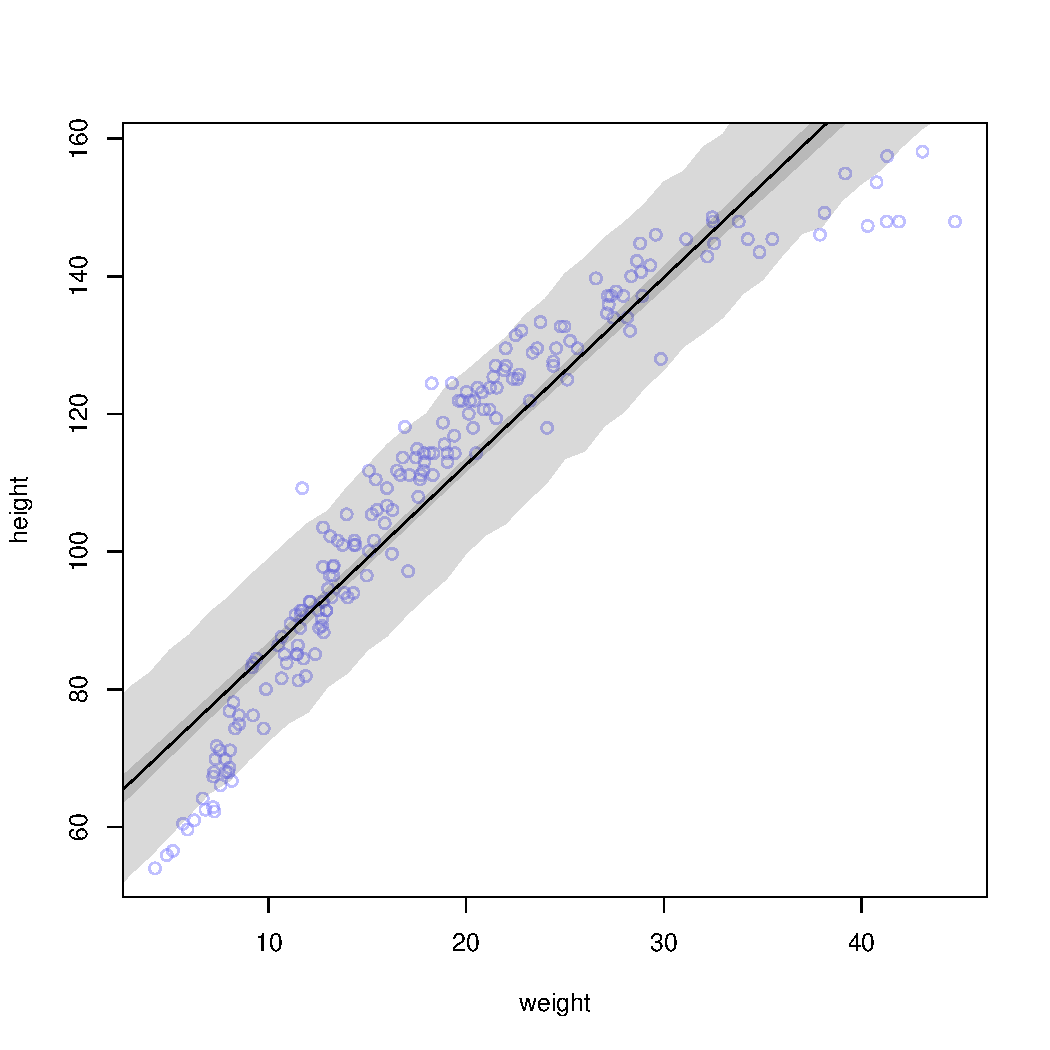
\includegraphics[width=\maxwidth]{figure/unnamed-chunk-7-1} 

\end{knitrout}

\item The rate of height increase in relation to weight does not appear to be constant. Thus, the data may be better modeled by a quadratic or cubic function.
\end{enumerate}

\begin{problem}{4H3}
\text{}\\
Suppose a colleague of yours, who works on allometry, glances at the practice problems just above. Your colleage exclaims, "That's silly. Everyone knows that it's only the \textit{logarithm} of body weight that scales with height!" Let's take your colleague's advice and see what happens.
\begin{enumerate}[(a)]
\item Model the relationship between height (cm) and the natural logarithm of weight (log-kg). Use the entire Howell1 data frame, all 544 rows, adults and non-adults. Fit this model using quadratic approximation:
\begin{center}
h\textsubscript{i} $\sim$ Normal($\mu$\textsubscript{i}, $\sigma$)\\
$\mu$\textsubscript{i} = $\alpha$ + $\beta$log(x\textsubscript{i})\\
$\alpha$ $\sim$ Normal(178, 100)\\
$\beta$ $\sim$ Normal(0, 100)\\
$\sigma$ $\sim$ Uniform(0, 50)
\end{center}
where h\textsubscript{i} is the height of individual \textit{i} and w\textsubscript{i} is the weight (in kg) of individual \textit{i}. The function for computing a natural log in R is just log. Can you interpret the resulting estimates?
\item Begin with this plot:

\begin{knitrout}
\definecolor{shadecolor}{rgb}{0.969, 0.969, 0.969}\color{fgcolor}\begin{kframe}
\begin{alltt}
\hlkwd{plot}\hlstd{(height} \hlopt{~} \hlstd{weight,} \hlkwc{data} \hlstd{= Howell1,} \hlkwc{col} \hlstd{=} \hlkwd{col.alpha}\hlstd{(rangi2,}\hlnum{0.4}\hlstd{))}
\end{alltt}
\end{kframe}
\end{knitrout}

Then use samples from the quadratic approximate posterior of the model in (a) to superimpose on the plot: (1) the predicted mean height as a function of weight, (2) the 97\% HPDI for the mean, (3) the 97\% HPDI for predicted heights.
\end{enumerate}
\end{problem}

\begin{enumerate}[(a)]
\item

\begin{knitrout}
\definecolor{shadecolor}{rgb}{0.969, 0.969, 0.969}\color{fgcolor}\begin{kframe}
\begin{alltt}
\hlstd{Howell1}\hlopt{$}\hlstd{weight.log} \hlkwb{<-} \hlkwd{log}\hlstd{(Howell1}\hlopt{$}\hlstd{weight)}

\hlstd{m3} \hlkwb{<-} \hlkwd{map}\hlstd{(}
  \hlkwd{alist}\hlstd{(}
    \hlstd{height} \hlopt{~} \hlkwd{dnorm}\hlstd{(a} \hlopt{+} \hlstd{b}\hlopt{*}\hlstd{weight.log, sigma),}
    \hlstd{a} \hlopt{~} \hlkwd{dnorm}\hlstd{(}\hlnum{178}\hlstd{,} \hlnum{100}\hlstd{),}
    \hlstd{b} \hlopt{~} \hlkwd{dnorm}\hlstd{(}\hlnum{0}\hlstd{,} \hlnum{100}\hlstd{),}
    \hlstd{sigma} \hlopt{~} \hlkwd{dunif}\hlstd{(}\hlnum{0}\hlstd{,} \hlnum{50}\hlstd{)}
  \hlstd{),} \hlkwc{data} \hlstd{= Howell1)}

\hlkwd{print}\hlstd{(m3)}
\end{alltt}
\begin{verbatim}
## 
## Maximum a posteriori (MAP) model fit
## 
## Formula:
## height ~ dnorm(a + b * weight.log, sigma)
## a ~ dnorm(178, 100)
## b ~ dnorm(0, 100)
## sigma ~ dunif(0, 50)
## 
## MAP values:
##          a          b      sigma 
## -23.785521  47.075738   5.134498 
## 
## Log-likelihood: -1661.9
\end{verbatim}
\end{kframe}
\end{knitrout}

For every one unit increase in log-kg, height increases by about 47 cm. The intercept a is negative and thus is uninterpretable. This arises because log(0) is undefined and $\log(x) \to -\infty$ as $x \to 0$.

\item

\begin{knitrout}
\definecolor{shadecolor}{rgb}{0.969, 0.969, 0.969}\color{fgcolor}\begin{kframe}
\begin{alltt}
\hlkwd{plot}\hlstd{(height} \hlopt{~} \hlstd{weight,} \hlkwc{data} \hlstd{= Howell1,} \hlkwc{col} \hlstd{=} \hlkwd{col.alpha}\hlstd{(rangi2,}\hlnum{0.4}\hlstd{))}

\hlcom{#Define sequence of weights to compute predictions for}
\hlcom{#These values will be on the horizontal axis}
\hlstd{weight.seq} \hlkwb{<-} \hlkwd{seq}\hlstd{(}\hlkwc{from} \hlstd{=} \hlnum{1}\hlstd{,} \hlkwc{to} \hlstd{=} \hlnum{70}\hlstd{,} \hlkwc{by} \hlstd{=} \hlnum{1}\hlstd{)}

\hlcom{#Use link to compute mu for each sample from the posterior}
\hlcom{#and for each weight in weight.seq}
\hlstd{post} \hlkwb{<-} \hlkwd{extract.samples}\hlstd{(m3)}
\hlstd{mu.link} \hlkwb{<-} \hlkwa{function}\hlstd{(}\hlkwc{weight}\hlstd{) post}\hlopt{$}\hlstd{a} \hlopt{+} \hlstd{post}\hlopt{$}\hlstd{b}\hlopt{*}\hlkwd{log}\hlstd{(weight)}
\hlstd{mu} \hlkwb{<-} \hlkwd{sapply}\hlstd{(weight.seq, mu.link)}

\hlcom{#Summarize the distribution of mu}
\hlstd{mu.mean} \hlkwb{<-} \hlkwd{apply}\hlstd{(mu,} \hlnum{2}\hlstd{, mean)}
\hlstd{mu.HPDI} \hlkwb{<-} \hlkwd{apply}\hlstd{(mu,} \hlnum{2}\hlstd{, HPDI,} \hlkwc{prob} \hlstd{=} \hlnum{0.97}\hlstd{)}

\hlcom{#Simulate heights from the posterior}
\hlstd{sim.height} \hlkwb{<-} \hlkwd{sim}\hlstd{(m3,} \hlkwc{data}\hlstd{=}\hlkwd{list}\hlstd{(}\hlkwc{weight.log}\hlstd{=}\hlkwd{log}\hlstd{(weight.seq)))}
\end{alltt}
\begin{verbatim}
## [ 100 / 1000 ]
[ 200 / 1000 ]
[ 300 / 1000 ]
[ 400 / 1000 ]
[ 500 / 1000 ]
[ 600 / 1000 ]
[ 700 / 1000 ]
[ 800 / 1000 ]
[ 900 / 1000 ]
[ 1000 / 1000 ]

\end{verbatim}
\begin{alltt}
\hlcom{#Summarize the simulated heights}
\hlstd{height.PI} \hlkwb{<-} \hlkwd{apply}\hlstd{(sim.height,} \hlnum{2}\hlstd{, PI,} \hlkwc{prob}\hlstd{=}\hlnum{0.97}\hlstd{)}

\hlcom{#Draw MAP line}
\hlkwd{lines}\hlstd{(weight.seq, mu.mean)}

\hlcom{#Draw HPDI region for line}
\hlkwd{shade}\hlstd{(mu.HPDI, weight.seq)}

\hlcom{#Draw PI region for simulated heights}
\hlkwd{shade}\hlstd{(height.PI, weight.seq)}
\end{alltt}
\end{kframe}
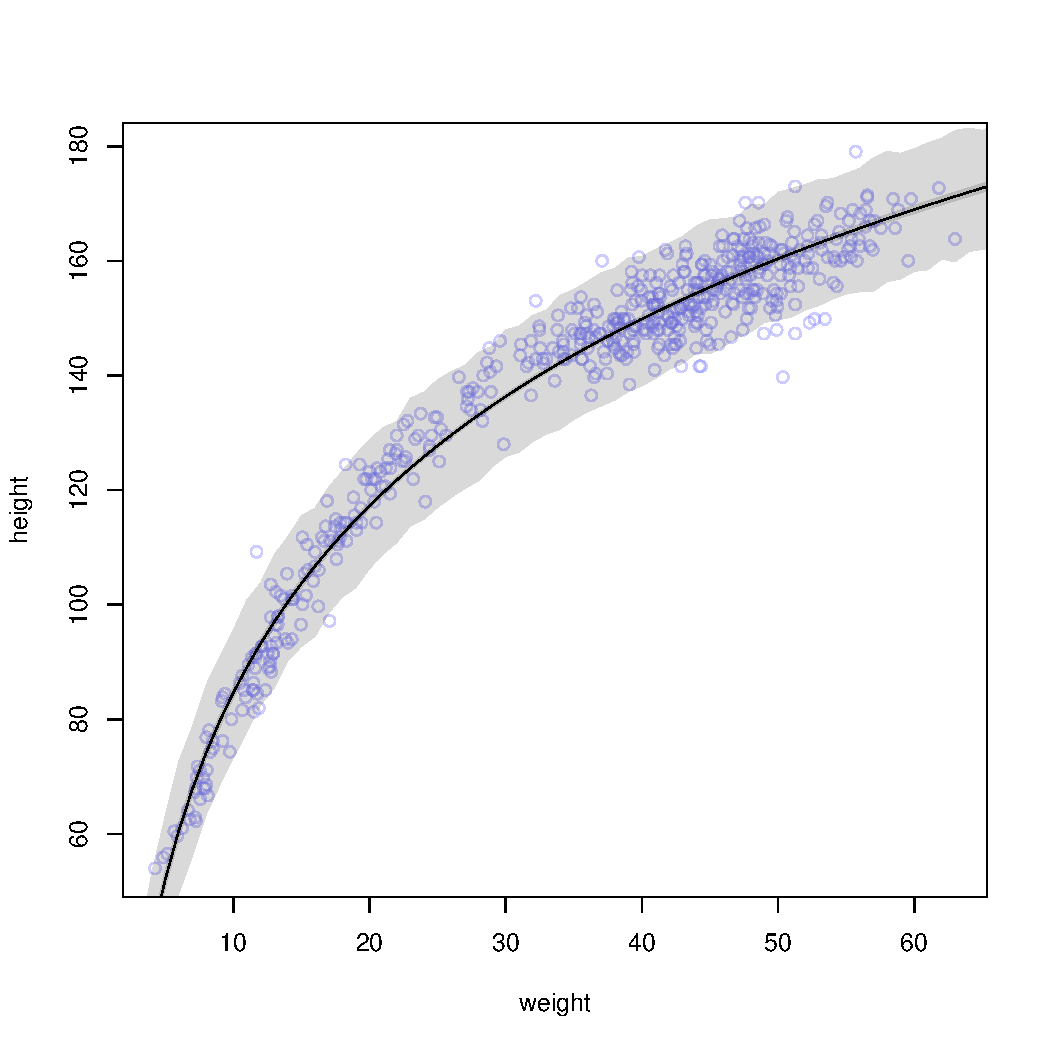
\includegraphics[width=\maxwidth]{figure/unnamed-chunk-10-1} 

\end{knitrout}


\end{enumerate}

\end{document}
